% "Who Verifies the Agents?" @ NeurIPS 2026 --- submission mode (double-blind).
% Content contract: CLAIMS.md --- every number below carries a C<n> tag in a margin
% comment; a number without one is a defect. Camera-ready: [final] is set; the
% submitted anonymous version is tagged workshop-submission in git.
\documentclass{article}
\usepackage[dblblindworkshop,final]{neurips_2026}
\workshoptitle{Who Verifies the Agents? Toward Reliable Agent Development}

\usepackage[utf8]{inputenc}
\usepackage[T1]{fontenc}
\usepackage{array}      % >{\raggedright} p-columns: justified narrow columns space badly
\usepackage{booktabs}
\usepackage{capt-of}   % \captionof: number the tables without floating them
\usepackage{graphicx}
\usepackage{amsmath,amssymb}
\usepackage{microtype}
\usepackage{xcolor}
\usepackage{hyperref}   % checklist.tex uses \url

\newcommand{\eps}{\varepsilon}

% Internal audit tags. Every quantitative sentence names the claim it rests on in
% paper/workshop/CLAIMS.md, which is checked mechanically. The tags are for the
% authors, not the reader: `make pdf` hides them, `make pdf-audit` shows them.
\newif\ifclaimtags\claimtagsfalse
\IfFileExists{.claimtags}{\claimtagstrue}{}
\newcommand{\ct}[1]{\ifclaimtags\hfill{\scriptsize\textcolor{gray}{[#1]}}\fi}

\title{Asserted Zeros: When a Valid Guarantee Certifies\\an Unmeasured Quantity}

\author{Zayyan Ahmed\\
  School of Electrical Engineering and Computer Science\\
  National University of Sciences and Technology (NUST), Islamabad, Pakistan\\
  \texttt{zahmed.bscs23seecs@seecs.edu.pk}}

\begin{document}
\maketitle

\begin{abstract}
A distribution-free guarantee certifies whatever score it is handed, including one that was never measured. We call this a \emph{measurement-integrity
failure}, and document one in a pipeline whose two LLM judges grade spoken answers.
It stored option probabilities to five decimals, so anything below
$5\times10^{-6}$ became exactly $0.0$, and rescaling what survived to sum to one
pushed the one remaining option (usually the correct one) to $1.0$. A record's
score is one minus the true answer's stored probability, so on 90.6\% of
graded records that score was exactly $0.0$: a certainty no judge expressed.
Those scores became the held-out set that fixes the release threshold, as
conformal prediction does. You sort them, take the one sitting at a position your error budget picks, and release an
option whose score falls at or below it. With nine in ten at the manufactured $0.0$, that position lands among them, so the threshold is $0.0$ and the gate admits exactly the options a judge
rounded up to $1.0$. It now turns on whether the two judges rounded up to the same option, not
on the evidence beneath them. A pre-registered probe found every grading decision we checked
unchanged. On the recordings this system actually ran, the gate released nothing
at all, with or without the defect. Re-imposed at that resolution on correctly measured scores, the
rounding makes the gate release more than measurement does in $36$ cases of $42$
and fewer in none,
certifying answers honest measurement would have withheld. The repair is dull: measure every option or refuse. Five questions about how
probabilities are recorded catch this before calibration.
\end{abstract}

\section{Introduction}\label{sec:intro}
Verification systems compose formal guarantees over quantities a model produces.
The guarantee is proved about a random variable; the system computes something it
takes to be that variable; and the composition is sound only if the two are the same. Verification
checks the guarantee against the score it was handed; nothing validates that the
score is the quantity intended. We show that they can differ: a guarantee can remain mathematically
valid while certifying a quantity that was never observed.
We call this a \emph{measurement-integrity failure}: the downstream guarantee
remains valid, but the quantity supplied to it is not the quantity the system
intended to measure. The category is broad: a verifier fed a truncated context measures every
probability correctly and still supplies the wrong conditional, so we say which member we demonstrate and which our diagnostic catches: a pipeline
\emph{recording a value it never observed}, because its record format has no way
to represent \emph{unmeasured}.

The setting is the one this workshop asks about: agentic systems delegate
consequential decisions to LLM verifiers, and a natural way to make that
verification \emph{reliable} is conformal prediction: calibrate a nonconformity score (ours is $1-p$ for an option, so a small score means a confident grader) on
held-out examples, release only when the calibrated uncertainty set is decisive \citep{vovk2005algorithmic,angelopoulos2023gentle}. The guarantee is
distribution-free and finite-sample, attractive precisely where verifier stakes
are highest. Our case study is a speech-based assessment verifier; the contribution is the
failure mode, not the domain.

That guarantee attaches to \emph{whatever score is fixed in advance}. Conformal validity says nothing about whether the score measures what its user thinks it
measures. Consider one record from our corpus. The verifier's recorded distribution over
$\{a,b,c\}$ was $\{1.0,\,0.0,\,0.0\}$, giving the true option a score of $1-1.0 = 0.0$: total certainty. Measured properly, the same model on the
same input gives $\{0.999998,\,1.35\times10^{-7},\,2.24\times10^{-6}\}$, a score
of $2.37\times10^{-6}$. Neither zero was observed, and neither was the $1.0$:
$0.999998$ rounded to five decimals \emph{is} $1.0$.\ct{C32, C66} One such record is a rounding curiosity. Ninety percent of them is a
calibration set whose defining feature, where its mass sits, is manufactured
(Figure~\ref{fig:scores}).

\begin{figure}[t]\centering
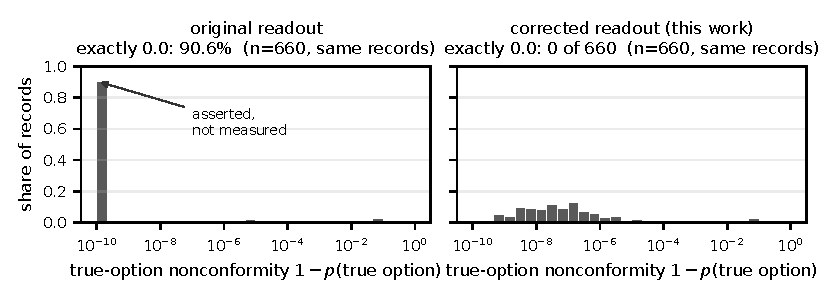
\includegraphics[width=\linewidth]{figs/fig_scores.pdf}
\caption{True-option nonconformity on the same $660$ graded records,
before and after. Left: the original readout, whose spike at exactly $0.0$ is
asserted, not measured. Right: the same records re-read by the corrected readout of
\S\ref{sec:fix}, same models, same prompt; $0$ of $660$ scores are exactly
zero (minimum $4.1\times10^{-10}$). Axes are shared, and exact zeros are drawn at the $10^{-10}$ axis
floor, since a log axis cannot show zero.\ct{C3, C77}}
\label{fig:scores}
\end{figure}

This failure needs only three properties, and none of them is exotic: a \emph{lossy record of a small probability} (a fixed-decimal writer that
rounds it away, a token matcher blind to the spelling it arrived under, a top-$k$
window that omits it, or any combination), \emph{renormalization over whatever is
left}, and a downstream consumer that treats the result as a
probability. None looks like a defect on its own; each is a reasonable local choice, and our own first repair of the writer re-introduced the same defect at
six decimals (\S\ref{sec:fix}). We read the source of three widely used option-scoring interfaces and one API
specification (Appendix~\ref{app:audit}): bounded visibility is documented, and
restricted-set normalization appears in the harnesses, legitimately there, since
the candidate set is enumerated by the task rather than lost, which is exactly what our case lacked. We claim nothing about
prevalence.

Conformal prediction is chosen precisely for its indifference to the model's probabilities: it needs no assumption that scores are calibrated or even meaningful, only exchangeable, and that immunity is what makes this failure
quiet: practitioners who adopt conformal methods \emph{because} confidences cannot
be trusted have little reason to audit them afterwards. The immunity covers
calibration, not measurement.

\textbf{The system.} Three corpora appear below (Table~\ref{tab:corpora}): the
artifact of \S\ref{sec:artifact} was found on two renderings of an $11$-item
work-readiness screener, and the corrected readout and cost analysis run on a
$10$-item civics corpus built after it, under the corrected readout from the start.

\begin{table}[t]
\caption{The corpora, in the order the work used them. All speech is
synthetic and degraded through telephone and noise channels. ``Graded'' counts
bank records with a scoring key; the screener records were written by the
original readout and later re-extracted under the corrected one.}\label{tab:corpora}
\centering\small
\begin{tabular}{llrrll}
\toprule
Corpus & Variation & Items & Options & Graded records & Used in \\
\midrule
Screener & channel, noise seed & $11$ & $3$ & $660$ of $770$ & \S\ref{sec:artifact}--\S\ref{sec:probe} \\
Screener & accented voice & $11$ & $3$ & $1{,}584$ of $1{,}848$ & \S\ref{sec:artifact}--\S\ref{sec:probe} \\
Civics (Powergrading) & speaker, channel & $10$ & $2$ & $13{,}992$ & \S\ref{sec:fix}--\S\ref{sec:cost} \\
\bottomrule
\end{tabular}
\end{table}

Four words carry the counting: an \emph{item} is one question of the
instrument in play; a \emph{record} is one channel rendering of
one spoken answer to one item; a \emph{session} is one speaker's full set of
answers; and the \emph{verdict} is the session-level pass/fail the decision rule
returns. Short written answers to civics questions (the Powergrading
corpus; \citealp{basu2013powergrading}) are spoken by synthetic voices
\citep{edgetts}, degraded through four channel conditions, and transcribed with
faster-whisper large-v3 \citep{fasterwhisper,radford2023whisper}. Two LLM judges, seated as \emph{judge} (Qwen3-32B-AWQ;
\citealp{qwen3report}) and \emph{evaluator} (Gemma-3-27B-IT;
\citealp{gemma3report}) and served by vLLM 0.25.1 \citep{kwon2023vllm}, then
grade each transcript independently, each with one decoding call whose first token is
read as the decision. Option probabilities are read from that token's
top-$k$ log-probabilities and combined across judges by minimum nonconformity; a
split-conformal threshold per item turns scores into per-item uncertainty sets;
and a deterministic validator (the \emph{gate}) \emph{releases} a verdict for a session, rather than withholding it, only if every combination
reachable from those sets yields the same verdict: equivalently, if the smallest and largest attainable totals fall on the same side
of the mark. That rule is a counting rule: pass if at least $6$ of the $10$ items
are correct; for a $k$-item subset the mark scales with $k$, so a single item is
its own decision. Per-item budgets compose by the union bound ($\Sigma\alpha = k\cdot\alpha_i$
at a common $\alpha_i$), and the exchangeability unit is the speaker;
Appendix~\ref{app:rule} gives the arithmetic.\ct{C38, C39, C41, C45}

The readout is lossy in three places: a fixed-resolution record, a token
matcher that recognizes only some spellings, and a shared window, which \S\ref{sec:artifact} takes apart. The window is shared with the whole
vocabulary: the constraint parameter our harness passed does not exist in the
serving stack's version and is silently ignored, so the corpus was extracted
unconstrained.\footnote{No recorded number is affected: masking shifts surviving
log-probabilities by a constant, so the renormalized distribution is invariant,
and the leading token is an option on $346$ of $347$ audited records
regardless.\ct{C64}}\ct{C62} The object of study is not the pipeline but the \emph{measurement} that
enters calibration.

\textbf{What conformal calibration does, and why an atom breaks it.} Split
conformal holds out examples whose answers are known, scores each one, sorts
those scores, and reads a threshold off the sorted list, the $\lceil(n{+}1)(1{-}\alpha)\rceil$-th, where $\alpha$ is the error budget its
user chooses. At test time an option joins the released set if its score falls
under that threshold, and a verdict is released only when the set is decisive.
The guarantee is real but narrow: coverage of at least $1-\alpha$ for
\emph{whatever score was fixed in advance}, assuming nothing about whether that
score is calibrated or even meaningful. That indifference is the method's
selling point, and exactly what makes this failure quiet: a threshold read off a sorted list is defenceless against a pile of identical values. When ninety
percent of the scores are the same manufactured $0.0$, the quantile lands inside
that pile and the gate stops responding to evidence, while every guarantee it
advertises still holds.

Two literatures ask whether a model's confidence can be \emph{trusted}; the
conformal literature offers guarantees that hold regardless. We ask a third question: whether the number recorded as a confidence was \emph{observed at all}, and show that when it was not, the guarantee is untouched, the judge's
decisions are unchanged, and the defect surfaces only in the calibration layer.
What we add is not the concept, which measurement theory and missing-data
statistics have long carried, but its instance: this failure inside a
distribution-free guarantee, whose own indifference to the score keeps it hidden.
The remedy is correspondingly boring: measure every option or refuse.

Concretely, we contribute:
\begin{enumerate}
  \item \textbf{An exact-zero artifact in a verification signal}
    (\S\ref{sec:artifact}): on $52.3\%$ of judge and $80.1\%$ of evaluator
    extractions only one option is left with a
    nonzero record, so its probability becomes $1.0$; under min-combination
    across two judges, $90.6\%$ of graded records' true-option scores are exactly
    $0.0$, and the calibrated threshold is exactly $0.0$ from
    $\alpha = 0.096$ upward. Re-running the original readout on a retained window separates the
    causes: repairing the five-decimal writer alone removes $7{,}733$ of them,
    the token matcher alone $256$, the top-$k$ window alone \emph{none}; counts that overlap rather than partition (Table~\ref{tab:blame}).
  \item \textbf{Correct measurement, independently checked} (\S\ref{sec:fix}): a
    readout that measures every option's probability or refuses (absence raises; full-precision serialization),
    validated on $13{,}992$ records ($0$ exact
    zeros) and, for both extractors, against a full-vocabulary reconstruction
    that shares neither its transport nor its window.
  \item \textbf{A pre-registered probe} (\S\ref{sec:probe}) separating what the
    artifact distorted (calibration inputs) from what it did not (argmax
    decisions), including the one substantive falsification and five vacuous ones at
    operating points where nothing releases; all ten are reported
    (Appendix~\ref{app:prereg}).
  \item \textbf{What it costs} (\S\ref{sec:cost}): re-imposing the defect on
    measured scores drives the calibrated threshold to an endpoint on every item
    it reaches, at every floor we tried. At the writer's own $5\times10^{-6}$,
    release rises in $36$ of the $42$ item-splits reached and falls in none, and
    on the split reported, wrong verdicts rise $57 \to 59$ (aggregate error is
    worse in $13$ of $20$ resplits). At $\tau = 10^{-2}$ it instead
    \emph{falls} ($19$ of $20$), so watching it would read the defect as an
    improvement (Appendix~\ref{app:ladder}).
  \item \textbf{A diagnostic another team can apply} (\S\ref{sec:takeaway}):
    five questions about a readout that expose the failure we demonstrate before
    its output reaches a calibration set, including the one our own defect got
    past.
\end{enumerate}
We frame this at the level of the workshop's question, the \emph{verification of the verifier's evidence}: the
gate went on returning well-formed verdicts while the evidence beneath them was
fabricated, with nothing in its behaviour to separate the two.

\section{The artifact: asserted zeros}\label{sec:artifact}
The two screener corpora of Table~\ref{tab:corpora} predate the civics corpus: the same $77$ spoken utterances under two
channel-and-voice draws (Appendix~\ref{app:corpora}).
The original readout took option probabilities from the single decision token's
top-$20$ log-probabilities, renormalized over the options present, and wrote the
result to JSON through Python's \texttt{round(p, 5)}. Three routes in that pipeline
reach the same record. An option can be absent from the window; present but
spelled in a way the reader's token matching does not recognize; or counted
correctly and still fall below $5\times10^{-6}$, which the serializer writes as
$0.0$. What unites them is not the window: \emph{a value that could not be
represented was written as the value zero}.

Which route acted is measurable, because the readout is re-runnable: we
re-extracted both corpora keeping the raw window, cut it to the top $20$ by
rank, aggregated under the old token matcher, renormalized, rounded to five decimals, and that reconstruction reproduces the recorded pattern of zeros on every record that has one. Two questions come apart, and only the second is causal: what did the reader have in hand when each zero was written, and what would
repairing one factor alone change?

\captionof{table}{Which factor erased each zero first, and which zeros repairing
that factor alone would remove. The columns count the same $7{,}861$ zeros and
must not be added: the left one partitions them, the right one cannot, since a
zero may be removable by several repairs or by none alone. ``First'' is pipeline
order: window, then token matcher, then writer.}\label{tab:blame}
\begin{center}\small
\begin{tabular}{lrr}
\toprule
Factor & Zeros it erased first & Zeros that repairing it alone removes \\
\midrule
Writer, five decimals & $7{,}733$ & $7{,}733$ \\
Token matcher, bare letters only & $97$ & $256$ \\
Window, top-$20$ rank cut & $31$ & $\mathbf{0}$ \\
\bottomrule
\end{tabular}
\end{center}

\noindent Every zero that some single repair removes is removed
by repairing the writer; the other $128$ need the writer \emph{and} a second
factor. Repairing the window removes not one of the $7{,}861$ zeros:
wherever an option fell outside it, the writer would have erased it anyway. The
rank window is not merely secondary but entirely preempted. The token matcher
is a real contributor: $97$
zeros where the option sat in the window under a spelling the reader could not
match, and $256$ that repairing it alone removes. This artifact is a record
format that could not represent a small probability, primarily by rounding it away, in a minority of cases by never counting it.\ct{C62, C69}

The consequence follows mechanically whichever route acted. When only one option is left
with a nonzero record, its probability becomes $1.0$, by renormalization where the others were never counted, by the writer where they were counted and rounded
away. The
record's resolution is the limit of what it can distinguish: across all $7{,}861$
recorded zeros we re-scored, the largest true probability behind one is
$1.84\times10^{-5}$ and the median is $2.55\times10^{-8}$. Nothing above $10^{-4}$ was ever hidden, but everything below the writer's precision was, and
that is exactly the range a calibration threshold reads.\ct{C67} On the two corpora that is
$52.3\%/51.4\%$ (judge) and $80.1\%/79.5\%$ (evaluator) of all extraction rows,
the two figures in each pair being the two corpora ($770$ and
$1{,}848$ rows).\ct{C1--C2, C62}

That is the per-judge picture. The pipeline then combines two separately-prompted
judges by minimum nonconformity ($s(o) = 1-p(o)$; $\min$ across judges), so
either judge collapsing to a one-hot on the true option forces the combined
true-option score to exactly $0.0$. On the graded records this occurs on $90.6\%/89.7\%$ of
rows, the spike visible in Figure~\ref{fig:scores}.\ct{C3} The combined share therefore exceeds either judge's own. The two judges are one model family per role, so their errors are correlated
and we do not predict the combined rate from the marginals.\ct{C52}

The calibration consequence is immediate: a split-conformal threshold is the
$\lceil(n{+}1)(1{-}\alpha)\rceil$-th order statistic of the calibration scores.
Once the zero count reaches that order statistic the threshold is exactly $0.0$: at a $90.6\%$ zero share, $\alpha \ge 0.096$; at $89.7\%$, $\alpha \ge
0.104$. Crossing it does not change the released set, since the five-decimal grid
leaves no score between $0$ and $10^{-5}$: an item's set holds
the options recorded at $1.0$ and excludes the rest.\ct{C4} A set that ends up empty is promoted to the full option set, withholding rather than asserting. At a threshold of $0.0$ the set is
therefore whichever options some judge scored $1.0$: a singleton when the judges'
one-hots agree, a doubleton when they disagree on a three-option item, and the
full set when neither survives.
The gate appears sharp; the sharpness is the artifact. 

We emphasize what this is not. It is not a violation of conformal validity: the coverage guarantee of \S\ref{sec:intro} holds here. What the artifact destroys is
its \emph{sharpness}. Exact coverage additionally requires a
continuous score distribution; ours carries an atom of $90.6\%$ at exactly
$0.0$, so realized coverage is pinned near $0.906$ for every $\alpha$ above the
crossover: conservative, and nearly insensitive to the budget its user chose.
Ties are a known pathology, and smoothed conformal randomizes through them by
construction \citep{vovk2005algorithmic}; it would restore a non-degenerate
threshold here without restoring any evidence, since the atom it spreads was
manufactured rather than observed.
And $0.906$ is not a calibration property: at threshold $0$ the true option
is covered exactly when some judge recorded it at $1.0$, so coverage is the rate
at which a grader's survivor is the truth. The gate has become a detector of
grader agreement.\ct{C4} Nor is it usefully described as an implementation bug, though it began as
one: everything downstream (thresholds, set sizes, release decisions) inherited a rounded, renormalized window while remaining formally correct. The defect is
invisible to conformal machinery because it is upstream of it, and to
ordinary testing because, as \S\ref{sec:probe} shows, it changes almost nothing
a system's behaviour would reveal.

\section{Measuring instead of asserting}\label{sec:fix}
The corrected readout makes one decoding call per record and
computes each option's probability as the \emph{sum over its token variants}
(``a'', ``A'', `` (a)'', ``a.'')\ in the decision token's top-$k$ ($k{=}100$),
since a model spells one choice several ways and any single spelling
understates it. Two hard guards define the semantics: (i) an option with no
variant anywhere in the window raises an error: absence is never recorded as zero, which was the equation that produced the artifact of
\S\ref{sec:artifact}; (ii) the
unnormalized option mass is persisted, so the residual carried by non-option
tokens is visible rather than silently absorbed. The score is computed on the
renormalized distribution; the unnormalized mass is recorded beside it and never
enters the score.\ct{C6, C40}

The refusal rate is the natural cost of ``measure or refuse'', so we report it:
zero. Both caches hold exactly $13{,}992$ rows and the probe holds no unscoreable records, a check rather than an assertion, since the readout raises and nothing catches it, so one refusal would have
halted the run mid-file.\ct{C37}

Two incidents in our own deployment show how easily this defect is
re-introduced, even by a team actively looking for it. First, the decoding
constraint we believed we were imposing never was: our harness passed a parameter
name the serving stack had retired, and unknown parameters are ignored at every
arity rather than rejected, so the readout measured an unconstrained model
throughout.\ct{C64} A readout that scores each option in its own call (how we first rebuilt it) inherits that assumption and fabricates a
plausible near-uniform distribution, silent exactly in the
borderline band that decides calibration; an identity guard (the emitted token must equal the option asked for) turned ${\sim}28{,}000$ would-be silently wrong
scores into one diagnosed defect.\ct{C7} Second, our own first writer rounded to
six decimals, returning a measured $4.3\times10^{-7}$ as exactly $0.0$ on disk:
\emph{the same defect as \S\ref{sec:artifact}, re-manufactured by the fix
itself}. A smoke test caught it; a regression test pins it now. That is no coincidence: the writer is the dominant route into the original artifact too, and it
returned the moment we stopped watching.\ct{C12, C62}

We then built the civics corpus (Table~\ref{tab:corpora}) \emph{under the measured readout from
the start}: $350$ synthetic speakers $\times$ $10$ items $\times$
$4$ channel conditions, less two unspeakable
responses disclosed in the pre-registration, graded by the same two blind judges. The \emph{same-record} before/after lives in Figure~\ref{fig:scores} and the probe
of \S\ref{sec:probe}; re-extracting the original corpora under the corrected
readout leaves $0$ of $660$ (and $0$ of $1{,}584$ on the second corpus) at
exactly zero, from minima of $4.1\times10^{-10}$ and $5.2\times10^{-10}$. It is the substrate for \S\ref{sec:cost}. Under
the measured readout: exactly-zero true-option scores number
$0/13{,}992$; no option is recorded at exactly $1.0$; per-extractor
minimum probabilities are $7.8\times10^{-9}$ and $3.9\times10^{-9}$; and the
unnormalized option mass separates the judges: the first never records below
$0.99$ (minimum $0.99987$), the second has a real tail ($36$ values below $0.9$,
minimum $0.4379$), so where variants leave mass elsewhere, the readout now says
so instead of absorbing it.

We can also report where the options sat in the
window: on an audited sample of each extractor, each
option's \emph{best-spelled} variant has median rank $2$ or better, never
exceeds $4$, and none of the $1{,}388$ ranks falls outside a top-$20$
window (a statement about where an option is \emph{findable}; most individual
spellings sit far lower). For this extractor on this
two-option corpus, then, a rank cut at $20$ could not have produced the artifact at all: the same negative result \S\ref{sec:artifact} reaches on the
three-option corpora, where repairing the window removes none of the zeros.\ct{C8--C11, C44, C63}

\textbf{Checking the fix against something other than itself.} A readout that
validates only against its own output is exactly what this paper warns about, so
for \emph{both} extractors we reconstructed the same quantity from the full
vocabulary, outside any server, on $347$ records each
(Appendix~\ref{app:recon}). Four predictions were registered before the
measurement; all four held on both. Option mass agrees with the deployed readout
to a median ratio of $1.000000$ ($99$th-percentile deviation $0.013$ evaluator,
$6.6\times10^{-7}$ judge); scores agree to median ratios of $1.000000092$ and
$1.000000000$, every one within a factor of two; no score is exactly zero; and
the spellings the readout aggregates over carry all but $6\times10^{-12}$
(evaluator) and $2.3\times10^{-7}$ (judge) of the option mass.

Four limits. The reconstruction runs on the
deployment's inference engine, so it validates the \emph{readout}, not the engine
or serving stacks we did not use. It shares the
corrected readout's token matcher, so it cannot detect a spelling that matcher misses; that
class is bounded separately, by enumerating the vocabulary for option spellings
the matcher rejects. Those missed spellings carry more mass on the judge than the evaluator ($2.3\times10^{-7}$ against $6\times10^{-12}$, above the smallest option probabilities we report), but on no record does that mass reach the
smallest option's own, at worst $13\%$ of it. And on a deliberately
adversarial stratum the evaluator's agreement loosens by an order of magnitude
(mass ratios $0.90$ to $1.16$) while the judge's does not; we report that stratum
apart rather than pooling it into the headline.\ct{C60, C61, C72, C73}

\section{A pre-registered probe: what the artifact did and did not
distort}\label{sec:probe}
Ten predictions are registered across two documents ($4+6$), and all
ten are reported: four held, one was substantively falsified, and five were
falsified \emph{vacuously}, at registered operating points where nothing releases
at all (Appendix~\ref{app:prereg}). Both, one for the probe below and one for the corpus of \S\ref{sec:fix}, were frozen before the harness that scores
them existed, an ordering visible in the artifact's history and timestamped by
our own record-keeping rather than a third party. The one that carries weight here is the corpus
document's fourth, registered before the corpus existed: that after the fix the
share of calibration scores at exactly $0.0$ would fall below $0.20$ (from
${\sim}0.90$) and the calibrated threshold would be strictly positive in every
split seed. It held, its operating points amended before scoring
(Appendix~\ref{app:prereg}).\ct{C19, C43}

Before re-extraction we froze four predictions about what correct measurement
would change on the \emph{original} corpora ($200$ records each, both judges,
stratified by \emph{recorded support}: the number of options recorded nonzero,
so support-1 rows are exactly those collapsed to a one-hot).\ct{C18} Three held;
one failed; we report all four. They were not independent: Q1 is close to forced
by the fix and Q4 follows from it; Q2 and Q3 were the two genuinely at
risk.

\textbf{Held.} Q1: on every support-1 row whose surviving option was the true
one, the measured score is strictly positive ($100/100$, $156/156$, $99/99$,
$162/162$ across pool$\times$judge): the zero was always an artifact. Q3: argmax decisions are robust: $0/200$ flips on every stratum, which bounds the flip rate on the
probed sample at $1.5\%$ (exact one-sided $95\%$; the rule of three). We do not
extrapolate that bound to the full corpus: the probe was stratified by recorded
support and drawn from the original corpora, so it is not a random sample of
anything larger. ``Unchanged'' is what we observed, not what the probe
guarantees.\ct{C51} Q4: the calibration dial comes alive: the $\alpha{=}0.1$ threshold moves from $0.0$ to $1.3\times10^{-3}$
($1.7\times10^{-4}$ on the second corpus), both on the probe's stratified
$200$-record sample, an illustration of the dial rather than an operating point, with zero-score share ${\sim}0.90 \to 0.000$.\ct{C13, C15--C16}

\textbf{Failed.} Q2 predicted the measured distributions would differ
substantially in total variation (median TV $\ge 0.05$ on support-1 rows).
Measured: median TV runs $4.2\times10^{-8}$ to $1.1\times10^{-4}$ across
corpus, extractor and stratum: falsified by two to six orders of magnitude.\ct{C14}
The prediction mistook a missing option for missing mass: the options that went
missing were small (the largest true probability behind any zero is
$1.84\times10^{-5}$, \S\ref{sec:artifact}), and removing small mass barely moves
a distribution.
This falsification is the sharpest result of the four: the artifact barely moved the distribution's \emph{bulk}; what it destroyed
was the \emph{tail}. The practical
reading is uncomfortable for downstream users: a system built on the original readout makes the same decisions and reports
the same argmaxes, so nothing in its behaviour signals that its calibration layer
is consuming fabricated evidence. The artifact is invisible except where it acts.

Stated plainly: the original readout was accurate to about $10^{-6}$ nearly
everywhere, and its whole defect was writing an exact $0$ where the truth was
around $10^{-6}$. That sounds negligible, and for the model's decisions it is, but not for calibration, for the reason \S\ref{sec:intro} gives.\ct{C17}

\section{What the artifact costs at the gate}\label{sec:cost}
The probe says the artifact is hard to see. This section asks what it does, by
re-imposing the readout's own equation on the measured scores of the binary
corpus of \S\ref{sec:fix}: record any option below a floor $\tau$ as $0.0$,
renormalize, and hold the records, the split, the calibration and the decision
rule fixed. This is a controlled simulation of the mechanism and is \emph{not}
pre-registered. The shape is right: a fixed-decimal writer zeroes
every probability below its resolution, so the original defect \emph{was} a
probability floor, at $5\times10^{-6}$, and this re-imposes the same operation, at that setting and coarser ones. It does not model either other route: the token matcher drops mass rather
than rounding it, and the rank route removes no zeros when repaired
(Table~\ref{tab:blame}) and is inert here anyway. At the writer's own $5\times10^{-6}$ the floor already zeroes $53.1\%$ of
calibration scores and already issues wrong verdicts measurement does not
($57 \to 59$), while no item loses all its release. The figures below use
$\tau = 10^{-2}$, a coarser setting that shows the mechanism's shape;
Appendix~\ref{app:ladder} runs the ladder between them. Two harms follow, and
they scale differently. The budget dial dies: wherever the floor reaches an item
the threshold sits on an endpoint, at every floor we tried. And the gate issues
wrong verdicts measurement withholds: two more at the writer's own floor on the
split reported, five at $10^{-2}$.\ct{C33, C46, C62, C70, C71, C81}

\textbf{Where truncation acts, it drives the threshold to an endpoint.} A floor rewrites only the scores beneath it, so it misses some items: on four of
the ten here (calibration error $0.060$--$0.069$; median three across the
resplits below) enough of the calibration sample
already sits above $\tau$ that the quantile never moves, and threshold, release
set and error count are bit-identical to the measured gate. Truncation is not uniform; it reaches items whose evidence was concentrated
enough for a floor to reshape.

Where it does reach, most of the calibration sample collapses onto $0$ or $1$ and
the $(1{-}\alpha_i)$ quantile lands in the mass the floor created, so the
threshold takes one of two values and a single comparison decides which. The
threshold is $0$ exactly when at least $\lceil (n{+}1)(1{-}\alpha_i) \rceil =
106$ of the $116$ calibration scores are zero: equivalently, in the collapsed regime where the
floor has driven every reached score to $0$ or $1$, when both judges miss on at most \emph{ten} of them. The count is the invariant, not the rate: the
speaker-level split leaves $n_{\text{cal}} \in \{115,116,117\}$ and the order
statistic allows exactly ten at each, so $10/116 = 0.086$ is this split's
instance of a threshold that moves slightly with $n$. Below that line (the \emph{step}), the gate admits every option the
readout zeroed: release rises on all four items concerned, and it rises
\emph{including on sessions the system gets wrong}. Above it the quantile falls in the mass at one, every set is
full, and the gate releases nothing at all. Figure~\ref{fig:step} shows both
regimes at $\Sigma\alpha = \alpha_i = 0.10$, with the collapse falling between
the items at error $0.069$ and those at $0.155$, consistent with a step at $0.086$, though ten items cannot separate $0.086$ from $\alpha_i$ itself, and we
claim only that the step lies where the order statistic requires.\ct{C47}

\begin{figure}[t]\centering
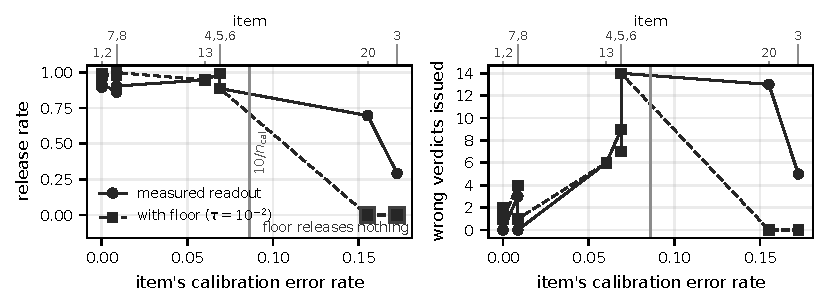
\includegraphics[width=\linewidth]{figs/fig_stepfunction.pdf}
\caption{Ten single-item decisions at an honest budget ($\Sigma\alpha =
\alpha_i = 0.10$, telephone stratum, $n_{\text{test}}{=}116$), with the floor re-imposed at $\tau = 10^{-2}$ (coarser than the
five-decimal writer's own $5\times10^{-6}$; Appendix~\ref{app:ladder} runs the
ladder), ordered by calibration error rate: the share of calibration records both judges score below $0.5$ for the true option, a close proxy for the share the floor zeroes ($1.57\%$ of records fall between $\tau$ and $0.5$; rates are channel-driven, Appendix~\ref{app:corpora}).\ct{C94} The vertical line is the step,
at ten wrong of $n_{\text{cal}}$. The floor reaches six of the ten: above the step it releases
nothing (marked), and on the four below it releases more than measurement does, extra certificates that are not free (right panel). The other four keep
enough calibration mass above $\tau$ that the quantile never moves, so the two readouts coincide exactly.
At the writer's own $5\times10^{-6}$ the floor changes two items, none loses its
release, and wrong verdicts rise $57 \to 59$ (Appendix~\ref{app:ladder}, Table~\ref{tab:ladder}).\ct{C47, C48}}
\label{fig:step}
\end{figure}

\textbf{Certificates the measurement does not issue.} Each is a single-item decision, so a release is a verdict the system issues. Below the step, truncation issues wrong verdicts that measurement does
not: items~1, 2 and~8 go from $0$ to $2$, $1$ and $1$, item~7 from $3$ to
$4$.\ct{C48} At the writer's own $5\times10^{-6}$ item~1 still goes from $0$ to $2$;
it is the floor's whole cost there. This is the paper's title under a controlled floor: a guarantee that
remains valid, certifying sessions on probabilities that were never
observed. Above it, at this floor, the harm runs the other way: items~20 and~3 (pool IDs, not ranks) lose all $81$ and all $34$ of their releases, so a floor coarse enough to reach
them makes the gate useless on hard items and reckless on easy ones.

\textbf{When aggregate monitoring would not catch it.} Summed over the ten
decisions at $\tau = 10^{-2}$, wrong verdicts \emph{fall} under truncation, $57$
to $44$, because the two high-error items stop releasing at all: a practitioner
watching aggregate error would see improvement while per-item behaviour became
arbitrary.\ct{C49} The inversion belongs to the coarse floor: at the writer's
own $5\times10^{-6}$ aggregate error is \emph{worse} in $13$ of
$20$ resplits; the sign flips only once the floor silences the hard items.\ct{C92}

\textbf{What survives resampling, and what does not.} These counts come from one split, at an $n_{\text{cal}}$ where
\S\ref{sec:related} puts the training-conditional band at $1.4$--$2.5\times$, so we repeated the measurement over twenty speaker-disjoint resplits
of the same corpus (seeds $0$--$19$), which bounds split sensitivity rather than replicating; a third of each split, reserved for fitting a grader, is unused, leaving $n_{\text{cal}}$ and $n_{\text{test}}$ near $116$. At $\tau = 10^{-2}$ the threshold lands on an endpoint on
every item the floor reaches ($141/141$ item-splits), at least one item collapses
to zero release in $20/20$, and in $20/20$ at least one item below the step
issues a wrong verdict that measurement does not. At the writer's own $5\times10^{-6}$ the endpoint result survives ($42/42$) and so does the wrong verdict ($13/20$ splits, a different $13$ from the aggregate count above, release rising in $36$ of $42$ item-splits and falling in none); the collapse does not.\ct{C91, C92, C93}

Three things do not hold. The constants move (measured wrong verdicts $38$--$72$ across splits,
truncated $26$--$63$, so $57 \to 44$ is an instance, not an estimate), and at $10^{-2}$ release below the step does not always rise: of the $117$ item-splits where the floor reaches an item below the step it rises in $105$, ties in $6$, falls in $6$, so at that floor we claim the endpoint, not a direction. Nor is the step's location a clean function of error rate: what decides it is where an item's score mass sits relative to $\tau$ (item $20$ at median error $0.134$ collapses in $19/20$ splits, item $3$ at $0.138$ in $5/20$). A fresh serving process reproduces every per-item threshold bit for bit, the inert and zero-release sets unchanged, one release count moving by one.\ct{C54, C55, C56, C57, C58, C59, C79}

\textbf{And at the deployed operating point, none of this is visible.} There the rule is $k{=}10$ at $\Sigma\alpha \le 0.5$, so $\alpha_i \le 0.05$,
and at $\alpha_i{=}0.01$ the order statistic $\lceil 115.83 \rceil = 116 = n$ is the
sample maximum for \emph{any} score distribution. On the mixed-condition stream
the system actually ran, nothing releases with or without the artifact, at any $\tau$ and every
registered budget. That is the stream's doing, not the budget's alone: on the telephone stratum at the same operating point, $32$ of $116$ sessions
release under measurement and none under the floor, a visible collapse.\ct{C50}

\section{Limitations and related work}\label{sec:related}
\textbf{Limitations.} At calibration $n{=}116$ a single split's realized rates
are measurements, not tests of the guarantee. Miscoverage conditional on one
calibration draw is Beta-distributed in $n$ and the order statistic alone
\citep{vovk2012conditional}, with a $95$th percentile at $2.5\times$, $2.0\times$ and $1.4\times$ nominal
for $\alpha = 0.01$, $0.02$, $0.10$: twice nominal is an ordinary draw at this $n$, not a property of our scores, and one to quote as a band.\ct{C29} 
Our corpora are synthetic-TTS speech over two assessment instruments with one
model family per seat, and the constants do not carry beyond them
(Appendix~\ref{app:repro} records how each is checked). The mechanism (a probability recorded through a representation that cannot
hold it, renormalized, then consumed as a calibration score) is not specific to
speech or assessment.\ct{C30} Appendix~\ref{app:audit} cuts the other way: what we found elsewhere was not what was causal here (repairing the window removes not one zero), and the mechanism behind most of our own zeros appeared in neither system that writes a
probability record. The failure is reachable, not
shown to be common.\ct{C62, C87, C88, C89}

\textbf{Related work.} Conformal prediction and its split form are classical
\citep{vovk2005algorithmic,angelopoulos2023gentle}; training-conditional validity is due to
\citet{vovk2012conditional}, risk control to \citet{angelopoulos2025learn}, and
class-conditional feasibility floors to \citet{ding2023class}. Conformal methods over LLM outputs typically consume log-probabilities as
scores \citep{kumar2023conformal,quach2024conformal}, credal-set predictors inherit coverage the same way
\citep{javanmardi2024credal}, and set-valued classification traces to
\citet{sadinle2019least}.

A second literature asks whether model confidences can be trusted at all:
networks are overconfident \citep{guo2017calibration}, language models carry
signal about their own correctness \citep{kadavath2022know}, verbalized
confidences can beat raw logits \citep{tian2023askcal}, and uncertainty over
generated text needs semantic equivalence \citep{kuhn2023semantic}. A third studies LLM verifiers themselves and their documented biases \citep{zheng2023judging,wang2024unfair}.

Older fields asked it first. Measurement theory separates the quantity
intended from the one an instrument delivers; construct validity \citep{cronbach1955construct} is the concern that a well-behaved instrument measures the wrong thing. Coding an absent value as zero is a missing-data mechanism, not at random
here: an option is dropped exactly when it is small
\citep{rubin1976inference}. The closest analogue is runtime verification, a trusted checker guarding an untrusted component \citep{sha2001simplex}.

\section{A diagnostic for measurement integrity}\label{sec:takeaway}
Measurement-integrity failures are hard to test for because they leave
behaviour intact: nothing in the stack raised an alarm. What can be tested is the
readout, and five questions expose the one we found.
\emph{Is every option's probability present in the window you read?} A
readout returning fewer options than exist is asserting the rest.
\emph{Do you keep the unnormalized mass?} Renormalizing without recording
what was renormalized destroys the evidence anything went missing.
\emph{Can you name a recorded probability you never observed?} A
measurement pipeline should be able to refuse; ours raises rather than write a
zero it never measured.
\emph{Can the format you write to represent the smallest probability you
can measure?} A window admitting every option is undone by a writer that rounds
what it admits: five decimals cannot express $10^{-7}$, and repairing that writer
alone removes $7{,}733$ of our $7{,}861$ zeros.
\emph{Does the emitted token match the one you asked for?} This catches a constraint passed but silently ignored, as ours was.

All five inspect the readout, which needs its code. The distribution it
produces needs only the scores: an atom like Figure~\ref{fig:scores}'s is visible
at a glance, and is the check a consumer of someone else's harness can still run.
These target the subclass we demonstrate: a value recorded without being
observed, not a readout that measures the wrong conditional correctly. Conformal prediction did not fail here. A valid guarantee is only as meaningful as the
measurement handed to it, and nothing inside checks the handoff.

\bibliographystyle{plainnat}
\bibliography{refs}

\appendix

\section{The decision rule, in full}\label{app:rule}
The release rule is a counting rule: a session passes if at least $6$ of its $10$
items are correct. For the $k$-item subsets used in \S\ref{sec:cost} the mark
scales as $\max(1,\mathrm{round}(6k/10))$, giving $1,1,2,3,6$ at
$k = 1,2,3,5,10$. Per-item budgets compose by the union bound: a session is
mis-set if any of its $k$ item sets is, so $\Sigma\alpha = \sum_i \alpha_i =
k\cdot\alpha_i$ at a common $\alpha_i$. This needs no independence between items,
which matters because ours are not independent. The exchangeability unit is the
speaker: splits are speaker-level, so no speaker's records straddle calibration
and test.\ct{C38, C39, C41, C45}

\section{The committed artifact}\label{app:repro}

Every quantitative claim in this paper is recorded against the committed artifact
it came from, and a build-time check re-reads the compiled PDF and requires each value printed
in the content pages to trace to one of those records; the figures are produced by
committed scripts that re-derive their headline shares from the artifacts on each
build. Code and data are released at \url{https://github.com/rainsfal1/asserted-zeros}.

All model serving runs on a single $46$\,GB GPU with one extractor resident at a
time; the two extraction passes over the binary corpus take under an hour in
total. Every other result in this paper is CPU-only arithmetic over the
committed score caches and re-runs in minutes, so the analysis reproduces
without a GPU.

A second fabrication path exists in the same code: if \emph{no} option survived
the window, a one-hot was fabricated on the emitted token. Its rate on the
original run is unmeasurable, because that run did not keep the window;
re-extracting the same records with the window kept bounds the opportunity
instead, and across all $5{,}236$ extractions there is none where the old reader
would have found nothing to renormalize. A real defect that never fired
here.\ct{C4--C5}

\section{Pre-registration bookkeeping}\label{app:prereg}
Of the ten registered predictions, five, all loop-policy predictions in the corpus document, were falsified \emph{vacuously}: at their registered operating points
nothing releases at all, for the reason \S\ref{sec:cost} gives and not because of
the loop, so we count them apart from the one substantive falsification (Q2 in \S\ref{sec:probe}): a prediction refuted by an inert operating point is
information about the configuration, not the hypothesis. The corpus document's fourth prediction had its scored operating points amended before
scoring, from $\Sigma\alpha \in \{0.05, 0.10\}$ to $\{0.10, 0.20\}$, because at
the lower budgets nothing releases and the prediction would have been decided by
arithmetic rather than evidence; the amendment is dated in the registered
document and is additions-only.\ct{C19, C43}

For completeness of the registration record, a third frozen document
(a feasibility-frontier study, five predictions) is registered in the artifact
and is not reported in this paper. It ships with the artifact;
its predictions are scored there.

\section{How the full-vocabulary reconstruction works}\label{app:recon}
For each sampled record we take the prompt the deployed extractor sent, assert
its token ids are identical to the server's own tokenization of the same
messages, and run one forward pass outside any server. The next-token distribution is read at the decision position over a
window of $2048$ of a $151{,}669$- and $262{,}145$-token vocabulary. Option mass
is the sum over all tokens that normalize to an option. Some option spellings
fall outside that window on every record, so tokens outside it are
\emph{bounded} rather than assumed zero: each contributes at most the window's smallest probability, giving
a relative bound of $1.45\times10^{-13}$ (evaluator) and $5.3\times10^{-11}$
(judge). The comparator is a fresh extraction from the same server instance rather than
the committed cache, because a long-running server does not reproduce its own earlier outputs exactly: $154$ of $200$ records bit-identical against the
day-old instance that wrote the cache, worst deviation $1.27\times10^{-2}$. A
clean relaunch, by contrast, reproduces the cache almost perfectly ($99.98\%$
and $99.62\%$ of $13{,}992$ rows bit-identical per extractor), so the
instability is within-lifetime state, not launch nondeterminism; the
same-instance comparator guards against both.\ct{C60, C61, C65, C72, C79, C80}

\section{The corpora of \S\ref{sec:artifact}}\label{app:corpora}
Both corpora serve an $11$-item spoken work-readiness screening instrument
(options a/b/c per item; the scoring key is transcribed from a deployed system
and pinned in the artifact). Utterances are rendered by synthetic voices
\citep{edgetts}, degraded, and transcribed with faster-whisper large-v3
\citep{fasterwhisper}. The first corpus: $77$ utterances ($66$ answer-bank,
$11$ clean probes) $\times$ $5$ channel levels (telephone band-limiting and additive noise at
signal-to-noise ratios $+5/0/-5/-10$\,dB) $\times$ $2$ noise seeds $= 770$ rows, of which $660$ are graded bank records. The second: the same
$77$ utterances $\times$ $8$ accented voices $\times$ $3$ levels (telephone;
SNR $0/-5$) $= 1{,}848$ rows, $1{,}584$ bank. The binary civics corpus of
\S\ref{sec:fix} uses $4$ channel draws (telephone; SNR $0/-5/-10$).\ct{C83} In \S\ref{sec:cost}, the per-item error rates that place an item above or below the step are themselves channel-driven: the share of calibration records both judges score below $0.5$ runs
$5.4\%$ to $42.9\%$ across our four conditions, tracking word-error rate
($1.15$ on those records against $0.094$ elsewhere), so the recording, not the grader alone, sets how much error a gate must tolerate.\ct{C21, C22}

\section{The $\tau$-ladder}\label{app:ladder}
\S\ref{sec:cost}'s figures use $\tau = 10^{-2}$. The same measurement at the
defect's own scale, on the same stream and split:

\captionof{table}{\S\ref{sec:cost}'s per-item measurement repeated at four
floors, including $5\times10^{-6}$, the writer's own resolution.}\label{tab:ladder}
\begin{center}\small
\begin{tabular}{lrrrr}
\toprule
$\tau$ & Cal.\ scores at $0.0$ & Gates changed & Zero-release & Wrong \\
\midrule
$0$ (measured) & $0\%$ & --- & $0$ & $57$ \\
$10^{-6}$ & $46.3\%$ & $1$ & $0$ & $57$ \\
$5\times10^{-6}$ (the writer's) & $53.1\%$ & $2$ & $0$ & $\mathbf{59}$ \\
$10^{-4}$ & $75.8\%$ & $3$ & $0$ & $60$ \\
$10^{-2}$ (\S\ref{sec:cost}) & $91.3\%$ & $6$ & $2$ & $44$ \\
\bottomrule
\end{tabular}
\end{center}

\noindent At the writer's own resolution the floor already zeroes half the
calibration mass and the gate already issues wrong verdicts that measurement
does not ($57 \to 59$); the zero-release collapse, and with it the fall in aggregate error that
makes the defect read as an improvement, appear as the floor coarsens. Repeating
\S\ref{sec:cost}'s twenty resplits at each rung gives the same separation:
endpoint thresholds at $27/27$, $42/42$, $58/58$ and $141/141$; no zero-release
item below $10^{-2}$; and aggregate error worse under the floor in $0$, $13$,
$15$ and $1$ of $20$ splits as $\tau$ coarsens. Post-hoc, as \S\ref{sec:cost}
states.\ct{C81, C91, C92, C93}

\section{A lightweight audit of related interfaces}\label{app:audit}
To ask whether the assumptions our failure needs are peculiar to us, we read the source of three widely used option-scoring interfaces and one API
specification on 2026-08-19. All four are moving targets and we did not record
the commits we read, so the reading is dated rather than pinned: a reader
cloning later may find any cell changed. The table records assumptions,
not defects. Restricting to an enumerated candidate set and
normalizing over it is correct where the measured quantity is explicitly conditional; that
is ordinary scorer behaviour and is not the failure this paper documents. We make no claim
about prevalence, and none about the correctness of any system below.

\captionof{table}{Four option-scoring interfaces, each read at the level its
Evidence column states: \mbox{[V]} we read the implementation, \mbox{[D]} we read
only documentation or a type declaration. A dash means the property was not
found on the path we read.}\label{tab:audit}
\begin{center}\footnotesize
% column widths + default tabcolsep run 9.6pt past \textwidth; tighten the gaps
% rather than the columns, which would only make the cells taller
\setlength{\tabcolsep}{4pt}
\begin{tabular}{@{}>{\raggedright\arraybackslash}p{2.1cm}>{\raggedright\arraybackslash}p{1.5cm}>{\raggedright\arraybackslash}p{1.9cm}>{\raggedright\arraybackslash}p{2.0cm}>{\raggedright\arraybackslash}p{1.7cm}>{\raggedright\arraybackslash}p{3.0cm}@{}}
\toprule
System & Evidence & Precision & Candidate visibility & Renormal.\ & Interpretation \\
\midrule
OpenAI chat API & spec text [D] & --- & capped at $20$ & --- & bounded visibility is documented in the specification at $20$, the same width we read \\[2pt]
\texttt{lm-eval-\allowbreak{}harness} & source [V] & full float in the record & exact (echo); raises on the chat path & over the task's choices & the restricted-set assumption exists, and is legitimate here: the choices are enumerated, so the value is conditional by construction \\[2pt]
\texttt{lighteval} & source [V] & full float in the record & --- & over the task's choices & likewise legitimate: the candidate set is defined by the task, not lost; no precision loss on the serialized record \\[2pt]
\texttt{inspect\_ai} & config [D], path [V] & --- & $0$--$20$ declared & none & the visibility limit exists in configuration; its multiple-choice path parses text and never consumes probabilities \\
\bottomrule
\end{tabular}
\end{center}

\noindent Two results are worth separating. Bounded visibility and restricted-set
normalization each appear outside our system, so the assumptions are not ours alone, though wherever we found the normalization, it was over a candidate set the
task enumerates, which is precisely what our case lacked. But the route that produced most of
our own zeros, a writer that cannot represent a small probability, appears in
\emph{neither} harness that writes a probability record: \texttt{lm-eval-\allowbreak{}harness}
and \texttt{lighteval} serialize in full float, and \texttt{inspect\_ai}'s
multiple-choice path writes none. And in one case the discipline
\S\ref{sec:fix} recommends is already practised: on its chat-completions path
\texttt{lm-eval-harness} raises rather than returning an approximation, giving the
unavailability of prompt log-probabilities as its reason. We report that as behaviour
only; the source says nothing about calibration, so we claim no shared
motivation.\ct{C85, C86, C87, C88, C89, C90}

\section*{NeurIPS Paper Checklist}

\begin{enumerate}

\item {\bf Claims}
    \item[] Question: Do the main claims made in the abstract and introduction accurately reflect the paper's contributions and scope?
    \item[] Answer: \answerYes{}
    \item[] Justification: The abstract's claims map one-to-one to \S2--\S5 and \S7, and every number in
    the content pages traces to a committed artifact via a claims table. One registered prediction was substantively falsified and five vacuously, at
    operating points where nothing releases; all ten are reported in \S4 and
    Appendix~\ref{app:prereg}.
    \item[] Guidelines:
    \begin{itemize}
        \item The answer \answerNA{} means that the abstract and introduction do not include the claims made in the paper.
        \item The abstract and/or introduction should clearly state the claims made, including the contributions made in the paper and important assumptions and limitations. A \answerNo{} or \answerNA{} answer to this question will not be perceived well by the reviewers. 
        \item The claims made should match theoretical and experimental results, and reflect how much the results can be expected to generalize to other settings. 
        \item It is fine to include aspirational goals as motivation as long as it is clear that these goals are not attained by the paper. 
    \end{itemize}

\item {\bf Limitations}
    \item[] Question: Does the paper discuss the limitations of the work performed by the authors?
    \item[] Answer: \answerYes{}
    \item[] Justification: \S6 states the training-conditional inflation ($1.4$--$2.5\times$ nominal $\alpha$ at $n{=}116$), the synthetic-TTS scope over two instruments, and that the mechanism is not specific to speech while the constants do not transfer and prevalence is not shown.
    \item[] Guidelines:
    \begin{itemize}
        \item The answer \answerNA{} means that the paper has no limitation while the answer \answerNo{} means that the paper has limitations, but those are not discussed in the paper. 
        \item The authors are encouraged to create a separate ``Limitations'' section in their paper.
        \item The paper should point out any strong assumptions and how robust the results are to violations of these assumptions (e.g., independence assumptions, noiseless settings, model well-specification, asymptotic approximations only holding locally). The authors should reflect on how these assumptions might be violated in practice and what the implications would be.
        \item The authors should reflect on the scope of the claims made, e.g., if the approach was only tested on a few datasets or with a few runs. In general, empirical results often depend on implicit assumptions, which should be articulated.
        \item The authors should reflect on the factors that influence the performance of the approach. For example, a facial recognition algorithm may perform poorly when image resolution is low or images are taken in low lighting. Or a speech-to-text system might not be used reliably to provide closed captions for online lectures because it fails to handle technical jargon.
        \item The authors should discuss the computational efficiency of the proposed algorithms and how they scale with dataset size.
        \item If applicable, the authors should discuss possible limitations of their approach to address problems of privacy and fairness.
        \item While the authors might fear that complete honesty about limitations might be used by reviewers as grounds for rejection, a worse outcome might be that reviewers discover limitations that aren't acknowledged in the paper. The authors should use their best judgment and recognize that individual actions in favor of transparency play an important role in developing norms that preserve the integrity of the community. Reviewers will be specifically instructed to not penalize honesty concerning limitations.
    \end{itemize}

\item {\bf Theory assumptions and proofs}
    \item[] Question: For each theoretical result, does the paper provide the full set of assumptions and a complete (and correct) proof?
    \item[] Answer: \answerNA{}
    \item[] Justification: The paper proves no theorems, and the training-conditional band is cited to prior work rather than re-derived. Two pieces of arithmetic are stated with their assumptions inline: the session-level union bound ($\Sigma\alpha = \sum_i \alpha_i$ over the ten per-item sets, requiring no independence) and the location of the truncated gate's step, which is a count rather than a rate ($\lceil (n{+}1)(1{-}\alpha_i)\rceil$ leaves at most ten wrong of $n_{\text{cal}}$, giving $10/116$ on the reported split), and which \S5 states conditional on the $\tau$-floor reaching the item at all.
    \item[] Guidelines:
    \begin{itemize}
        \item The answer \answerNA{} means that the paper does not include theoretical results. 
        \item All the theorems, formulas, and proofs in the paper should be numbered and cross-referenced.
        \item All assumptions should be clearly stated or referenced in the statement of any theorems.
        \item The proofs can either appear in the main paper or the supplemental material, but if they appear in the supplemental material, the authors are encouraged to provide a short proof sketch to provide intuition. 
        \item Inversely, any informal proof provided in the core of the paper should be complemented by formal proofs provided in appendix or supplemental material.
        \item Theorems and Lemmas that the proof relies upon should be properly referenced. 
    \end{itemize}

    \item {\bf Experimental result reproducibility}
    \item[] Question: Does the paper fully disclose all the information needed to reproduce the main experimental results of the paper to the extent that it affects the main claims and/or conclusions of the paper (regardless of whether the code and data are provided or not)?
    \item[] Answer: \answerYes{}
    \item[] Justification: \S2--\S5 disclose the transport, the guards, the corpus construction, the speaker-level split, the score definition, and the truncation sweep's parameters; the probe and the corpus were pre-registered with frozen designs, both registered documents ship in the artifact, and the amendment re-pointing the corpus document's fourth prediction to its scored budgets is dated in that document. The \S5 measurements are regenerated by \texttt{sweep\_per\_item.py}, \texttt{sweep\_split\_stability.py} and \texttt{tau\_ladder.py}; the figures by \texttt{fig\_scores.py} and \texttt{fig\_stepfunction.py}.
    \item[] Guidelines:
    \begin{itemize}
        \item The answer \answerNA{} means that the paper does not include experiments.
        \item If the paper includes experiments, a \answerNo{} answer to this question will not be perceived well by the reviewers: Making the paper reproducible is important, regardless of whether the code and data are provided or not.
        \item If the contribution is a dataset and\slash or model, the authors should describe the steps taken to make their results reproducible or verifiable. 
        \item Depending on the contribution, reproducibility can be accomplished in various ways. For example, if the contribution is a novel architecture, describing the architecture fully might suffice, or if the contribution is a specific model and empirical evaluation, it may be necessary to either make it possible for others to replicate the model with the same dataset, or provide access to the model. In general. releasing code and data is often one good way to accomplish this, but reproducibility can also be provided via detailed instructions for how to replicate the results, access to a hosted model (e.g., in the case of a large language model), releasing of a model checkpoint, or other means that are appropriate to the research performed.
        \item While NeurIPS does not require releasing code, the conference does require all submissions to provide some reasonable avenue for reproducibility, which may depend on the nature of the contribution. For example
        \begin{enumerate}
            \item If the contribution is primarily a new algorithm, the paper should make it clear how to reproduce that algorithm.
            \item If the contribution is primarily a new model architecture, the paper should describe the architecture clearly and fully.
            \item If the contribution is a new model (e.g., a large language model), then there should either be a way to access this model for reproducing the results or a way to reproduce the model (e.g., with an open-source dataset or instructions for how to construct the dataset).
            \item We recognize that reproducibility may be tricky in some cases, in which case authors are welcome to describe the particular way they provide for reproducibility. In the case of closed-source models, it may be that access to the model is limited in some way (e.g., to registered users), but it should be possible for other researchers to have some path to reproducing or verifying the results.
        \end{enumerate}
    \end{itemize}


\item {\bf Open access to data and code}
    \item[] Question: Does the paper provide open access to the data and code, with sufficient instructions to faithfully reproduce the main experimental results, as described in supplemental material?
    \item[] Answer: \answerYes{}
    \item[] Justification: Code and data are public at \url{https://github.com/rainsfal1/asserted-zeros}, containing the extraction harnesses, the committed score caches, the pre-registration documents, and the scripts that regenerate both figures and all three \S5 sweeps from those caches; the underlying short-answer corpus is publicly available.
    \item[] Guidelines:
    \begin{itemize}
        \item The answer \answerNA{} means that paper does not include experiments requiring code.
        \item Please see the NeurIPS code and data submission guidelines (\url{https://neurips.cc/public/guides/CodeSubmissionPolicy}) for more details.
        \item While we encourage the release of code and data, we understand that this might not be possible, so \answerNo{} is an acceptable answer. Papers cannot be rejected simply for not including code, unless this is central to the contribution (e.g., for a new open-source benchmark).
        \item The instructions should contain the exact command and environment needed to run to reproduce the results. See the NeurIPS code and data submission guidelines (\url{https://neurips.cc/public/guides/CodeSubmissionPolicy}) for more details.
        \item The authors should provide instructions on data access and preparation, including how to access the raw data, preprocessed data, intermediate data, and generated data, etc.
        \item The authors should provide scripts to reproduce all experimental results for the new proposed method and baselines. If only a subset of experiments are reproducible, they should state which ones are omitted from the script and why.
        \item At submission time, to preserve anonymity, the authors should release anonymized versions (if applicable).
        \item Providing as much information as possible in supplemental material (appended to the paper) is recommended, but including URLs to data and code is permitted.
    \end{itemize}


\item {\bf Experimental setting/details}
    \item[] Question: Does the paper specify all the training and test details (e.g., data splits, hyperparameters, how they were chosen, type of optimizer) necessary to understand the results?
    \item[] Answer: \answerYes{}
    \item[] Justification: \S3 gives the corpus construction (350 speakers $\times$ 10 items $\times$ 4 channel conditions, two judges) and \S5 the speaker-level calibration/test split ($n{=}116$ calibration records per item), the truncation parameter, and the budget; exact configurations are in the artifact.
    \item[] Guidelines:
    \begin{itemize}
        \item The answer \answerNA{} means that the paper does not include experiments.
        \item The experimental setting should be presented in the core of the paper to a level of detail that is necessary to appreciate the results and make sense of them.
        \item The full details can be provided either with the code, in appendix, or as supplemental material.
    \end{itemize}

\item {\bf Experiment statistical significance}
    \item[] Question: Does the paper report error bars suitably and correctly defined or other appropriate information about the statistical significance of the experiments?
    \item[] Answer: \answerYes{}
    \item[] Justification: \S5's headline counts come from a single deterministic speaker-level split, so the paper repeats the entire measurement over twenty speaker-disjoint resplits and reports the spread rather than error bars: which claims hold across all twenty ($141/141$ endpoint thresholds; $20/20$ zero-release; $20/20$ wrong certificates below the step), and which do not (wrong-verdict totals ranging $38$--$72$ measured and $26$--$63$ truncated; the aggregate drop reversing at one seed; release below the step falling rather than rising in $6$ of $117$ item-splits). \S6 gives the reason single-split rates cannot be read as tests of the guarantee (at this $n$ the training-conditional band runs $1.4$--$2.5\times$ nominal, \citealp{vovk2012conditional}), and the probe's one interval claim carries its exact bound ($0/200$ argmax flips, one-sided $95\%$ upper bound $1.5\%$).
    \item[] Guidelines:
    \begin{itemize}
        \item The answer \answerNA{} means that the paper does not include experiments.
        \item The authors should answer \answerYes{} if the results are accompanied by error bars, confidence intervals, or statistical significance tests, at least for the experiments that support the main claims of the paper.
        \item The factors of variability that the error bars are capturing should be clearly stated (for example, train/test split, initialization, random drawing of some parameter, or overall run with given experimental conditions).
        \item The method for calculating the error bars should be explained (closed form formula, call to a library function, bootstrap, etc.)
        \item The assumptions made should be given (e.g., Normally distributed errors).
        \item It should be clear whether the error bar is the standard deviation or the standard error of the mean.
        \item It is OK to report 1-sigma error bars, but one should state it. The authors should preferably report a 2-sigma error bar than state that they have a 96\% CI, if the hypothesis of Normality of errors is not verified.
        \item For asymmetric distributions, the authors should be careful not to show in tables or figures symmetric error bars that would yield results that are out of range (e.g., negative error rates).
        \item If error bars are reported in tables or plots, the authors should explain in the text how they were calculated and reference the corresponding figures or tables in the text.
    \end{itemize}

\item {\bf Experiments compute resources}
    \item[] Question: For each experiment, does the paper provide sufficient information on the computer resources (type of compute workers, memory, time of execution) needed to reproduce the experiments?
    \item[] Answer: \answerYes{}
    \item[] Justification: Appendix~\ref{app:repro} records the compute: one 46\,GB GPU serving each extractor sequentially, the two extraction passes under an hour in total, and every other result CPU-only arithmetic over the committed caches, re-runnable in minutes.
    \item[] Guidelines:
    \begin{itemize}
        \item The answer \answerNA{} means that the paper does not include experiments.
        \item The paper should indicate the type of compute workers CPU or GPU, internal cluster, or cloud provider, including relevant memory and storage.
        \item The paper should provide the amount of compute required for each of the individual experimental runs as well as estimate the total compute. 
        \item The paper should disclose whether the full research project required more compute than the experiments reported in the paper (e.g., preliminary or failed experiments that didn't make it into the paper). 
    \end{itemize}
    
\item {\bf Code of ethics}
    \item[] Question: Does the research conducted in the paper conform, in every respect, with the NeurIPS Code of Ethics \url{https://neurips.cc/public/EthicsGuidelines}?
    \item[] Answer: \answerYes{}
    \item[] Justification: The research conforms to the NeurIPS Code of Ethics: the corpora are synthetic speech over a published short-answer dataset and an answer bank authored for an 11-item screener (Appendix~\ref{app:corpora}), so no human subjects, no personal data and no capability release are involved.
    \item[] Guidelines:
    \begin{itemize}
        \item The answer \answerNA{} means that the authors have not reviewed the NeurIPS Code of Ethics.
        \item If the authors answer \answerNo, they should explain the special circumstances that require a deviation from the Code of Ethics.
        \item The authors should make sure to preserve anonymity (e.g., if there is a special consideration due to laws or regulations in their jurisdiction).
    \end{itemize}


\item {\bf Broader impacts}
    \item[] Question: Does the paper discuss both potential positive societal impacts and negative societal impacts of the work performed?
    \item[] Answer: \answerYes{}
    \item[] Justification: The paper's subject is a reliability failure in automated assessment, and \S1 and \S5 state the stake plainly: a gate can look more certain than its evidence supports, and at an honest budget it can issue verdicts that correct measurement would not. We claim no broader societal analysis than that.
    \item[] Guidelines:
    \begin{itemize}
        \item The answer \answerNA{} means that there is no societal impact of the work performed.
        \item If the authors answer \answerNA{} or \answerNo, they should explain why their work has no societal impact or why the paper does not address societal impact.
        \item Examples of negative societal impacts include potential malicious or unintended uses (e.g., disinformation, generating fake profiles, surveillance), fairness considerations (e.g., deployment of technologies that could make decisions that unfairly impact specific groups), privacy considerations, and security considerations.
        \item The conference expects that many papers will be foundational research and not tied to particular applications, let alone deployments. However, if there is a direct path to any negative applications, the authors should point it out. For example, it is legitimate to point out that an improvement in the quality of generative models could be used to generate Deepfakes for disinformation. On the other hand, it is not needed to point out that a generic algorithm for optimizing neural networks could enable people to train models that generate Deepfakes faster.
        \item The authors should consider possible harms that could arise when the technology is being used as intended and functioning correctly, harms that could arise when the technology is being used as intended but gives incorrect results, and harms following from (intentional or unintentional) misuse of the technology.
        \item If there are negative societal impacts, the authors could also discuss possible mitigation strategies (e.g., gated release of models, providing defenses in addition to attacks, mechanisms for monitoring misuse, mechanisms to monitor how a system learns from feedback over time, improving the efficiency and accessibility of ML).
    \end{itemize}
    
\item {\bf Safeguards}
    \item[] Question: Does the paper describe safeguards that have been put in place for responsible release of data or models that have a high risk for misuse (e.g., pre-trained language models, image generators, or scraped datasets)?
    \item[] Answer: \answerNA{}
    \item[] Justification: The paper releases no models and no data with misuse potential; the artifact is measurement code and score caches over synthetic speech (a published short-answer dataset and an authored answer bank).
    \item[] Guidelines:
    \begin{itemize}
        \item The answer \answerNA{} means that the paper poses no such risks.
        \item Released models that have a high risk for misuse or dual-use should be released with necessary safeguards to allow for controlled use of the model, for example by requiring that users adhere to usage guidelines or restrictions to access the model or implementing safety filters. 
        \item Datasets that have been scraped from the Internet could pose safety risks. The authors should describe how they avoided releasing unsafe images.
        \item We recognize that providing effective safeguards is challenging, and many papers do not require this, but we encourage authors to take this into account and make a best faith effort.
    \end{itemize}

\item {\bf Licenses for existing assets}
    \item[] Question: Are the creators or original owners of assets (e.g., code, data, models), used in the paper, properly credited and are the license and terms of use explicitly mentioned and properly respected?
    \item[] Answer: \answerYes{}
    \item[] Justification: All three existing assets are cited where used: the published short-answer corpus in \S1 and the TTS and transcription systems in Appendix~\ref{app:corpora}, each used under its stated terms. No proprietary asset is redistributed.
    \item[] Guidelines:
    \begin{itemize}
        \item The answer \answerNA{} means that the paper does not use existing assets.
        \item The authors should cite the original paper that produced the code package or dataset.
        \item The authors should state which version of the asset is used and, if possible, include a URL.
        \item The name of the license (e.g., CC-BY 4.0) should be included for each asset.
        \item For scraped data from a particular source (e.g., website), the copyright and terms of service of that source should be provided.
        \item If assets are released, the license, copyright information, and terms of use in the package should be provided. For popular datasets, \url{paperswithcode.com/datasets} has curated licenses for some datasets. Their licensing guide can help determine the license of a dataset.
        \item For existing datasets that are re-packaged, both the original license and the license of the derived asset (if it has changed) should be provided.
        \item If this information is not available online, the authors are encouraged to reach out to the asset's creators.
    \end{itemize}

\item {\bf New assets}
    \item[] Question: Are new assets introduced in the paper well documented and is the documentation provided alongside the assets?
    \item[] Answer: \answerYes{}
    \item[] Justification: The re-extracted score caches, the measurement readout and the pre-registration and probe harnesses are released in the public repository, documented as described in Appendix~\ref{app:repro}, with enough to regenerate every figure.
    \item[] Guidelines:
    \begin{itemize}
        \item The answer \answerNA{} means that the paper does not release new assets.
        \item Researchers should communicate the details of the dataset\slash code\slash model as part of their submissions via structured templates. This includes details about training, license, limitations, etc. 
        \item The paper should discuss whether and how consent was obtained from people whose asset is used.
        \item At submission time, remember to anonymize your assets (if applicable). You can either create an anonymized URL or include an anonymized zip file.
    \end{itemize}

\item {\bf Crowdsourcing and research with human subjects}
    \item[] Question: For crowdsourcing experiments and research with human subjects, does the paper include the full text of instructions given to participants and screenshots, if applicable, as well as details about compensation (if any)? 
    \item[] Answer: \answerNA{}
    \item[] Justification: No crowdsourcing and no human subjects: all speech is synthetic TTS over a published text corpus and an answer bank the authors wrote.
    \item[] Guidelines:
    \begin{itemize}
        \item The answer \answerNA{} means that the paper does not involve crowdsourcing nor research with human subjects.
        \item Including this information in the supplemental material is fine, but if the main contribution of the paper involves human subjects, then as much detail as possible should be included in the main paper. 
        \item According to the NeurIPS Code of Ethics, workers involved in data collection, curation, or other labor should be paid at least the minimum wage in the country of the data collector. 
    \end{itemize}

\item {\bf Institutional review board (IRB) approvals or equivalent for research with human subjects}
    \item[] Question: Does the paper describe potential risks incurred by study participants, whether such risks were disclosed to the subjects, and whether Institutional Review Board (IRB) approvals (or an equivalent approval/review based on the requirements of your country or institution) were obtained?
    \item[] Answer: \answerNA{}
    \item[] Justification: No human-subjects research was conducted, so no IRB approval applies.
    \item[] Guidelines:
    \begin{itemize}
        \item The answer \answerNA{} means that the paper does not involve crowdsourcing nor research with human subjects.
        \item Depending on the country in which research is conducted, IRB approval (or equivalent) may be required for any human subjects research. If you obtained IRB approval, you should clearly state this in the paper. 
        \item We recognize that the procedures for this may vary significantly between institutions and locations, and we expect authors to adhere to the NeurIPS Code of Ethics and the guidelines for their institution. 
        \item For initial submissions, do not include any information that would break anonymity (if applicable), such as the institution conducting the review.
    \end{itemize}

\item {\bf Declaration of LLM usage}
    \item[] Question: Does the paper describe the usage of LLMs if it is an important, original, or non-standard component of the core methods in this research? Note that if the LLM is used only for writing, editing, or formatting purposes and does \emph{not} impact the core methodology, scientific rigor, or originality of the research, declaration is not required.
    %this research? 
    \item[] Answer: \answerYes{}
    \item[] Justification: LLMs are the measured object throughout \S2 and \S3, the judge and evaluator whose scores are calibrated; separately, LLM coding assistance was used during development, and every reported number is produced by committed scripts run against committed artifacts rather than by any model.
    \item[] Guidelines:
    \begin{itemize}
        \item The answer \answerNA{} means that the core method development in this research does not involve LLMs as any important, original, or non-standard components.
        \item Please refer to our LLM policy in the NeurIPS handbook for what should or should not be described.
    \end{itemize}

\end{enumerate}

\end{document}
